\documentclass[10pt,a4paper]{article}
\usepackage[utf8]{inputenc}
\usepackage[russian]{babel}
\usepackage[OT1]{fontenc}
\usepackage{amsmath}
\usepackage{amsfonts}
\usepackage{amssymb}
\usepackage[dvipsnames]{xcolor}
\usepackage{graphicx}
\graphicspath{{Images/}}
\usepackage[left=2cm,right=2cm,top=2cm,bottom=2cm]{geometry}
\usepackage{calc}
\usepackage{wrapfig}
\usepackage{setspace}
\usepackage{indentfirst}
\usepackage{subfigure}
\usepackage{multirow}
\usepackage{amsfonts}
\usepackage{hyperref}
\hypersetup{
    pdfstartview=FitH,  
    linkcolor=black,
    urlcolor=red, 
    colorlinks=true,
    citecolor=blue}
\usepackage{tikz}
\usetikzlibrary{ decorations.markings}

\title{Семинар 2}
\date{\today}

\author{Варламов Антоний Михайлович}

\begin{document}
	\maketitle
	
	\section{Погрешности округления. Погрешности арифметики с плавающей точкой}
	
		Существуют различные типы данных:
		
		\begin{enumerate}
			\item Integer(целые числа) -- используется 4 байта/8 байт
			\item Real (действительные числа) -- используется 4 байта (single 
				precision) или 8 байт (double precision) (Альтернативные 
				названия -- float и double). Число хранится в виде:
				
				\begin{equation}
					a = \pm 2^{\pm e}\left(1 + f\right)
				\end{equation} 
				
				
				single precision: OFL = $10^{38}$
				
				double precision: OFL = $10^{324}$
				
				Представление чисел в компьютере -- дискретное. Плотность 
				распределения чисел непостоянна.
				
		\end{enumerate}
		
		Характерные особенности компьютерной арифметики:
		
		\begin{enumerate}
			\item $a := 0.1$ но $a \neq 0.1$
			
			\item $10^{20} + 1 = 10^{20}$
			
				$\left(10^{20} + 1\right) - 10^{20} = 0$
				
				$\left(10^{20} - 10^{20}\right) + 1 = 0$
				
				Данные следствия говорят о том, что ноль в компьютерном 
				представлении не единственен.
				
			\item Все числа в компьютере неточны. Степень неточности:
		
			\begin{equation}
				\delta a = \frac{\Delta a}{a} \leqslant 	
				\varepsilon_{\text{маш}}
			\end{equation}
			
			\item Все операции неточны. Для обозначения 
			"компьютерных" операций	используются символы операции 
			в кружке.
			
			\begin{equation}
				a \oplus b = \left(a + b\right)\left(1 \pm \delta
				\right)	
			\end{equation}
			
			Для анализа обычно используются два метода:
			
			\begin{itemize}
				\item[a] Все операции точны, но числа имеют 	
				погрешность.
				\item[б] Все операции неточны, но числа точны 
			\end{itemize}
			
			Рассмотрим пример применения разных методов:
			
			\begin{equation}
				a_{1} + a_{2} + a_{3}
			\end{equation}
			
			\begin{eqnarray}
				\left(a_{1} + a_{2}\right)\left(1 + \delta_{1}\right) \oplus a_{3} =\\ \left(\left(a_{1} + a_{2}\right)\left(1 + \delta_{1}\right) + a_{3}\right)\left(1 + \delta_{2}\right) =\\ a_{1} + a_{2} + a_{3} + \delta_{1}\left(a_{1} + a_{2}\right) + \delta_{1}\delta_{2}\left(a_{1} + a_{2}\right) + \delta_{2}\left(a_{1} + a_{2} + a_{3}\right) \approx \\a_{1} + a_{2} + a_{3} + a_{1}\left(\delta_{1} + \delta_{2}\right) + a_{2}\left(\delta_{1} + \delta_{2}\right) + a_{3}\delta_{2}
			\end{eqnarray}
		\end{enumerate}
		
		Вспомним прошлые результаты:
		
		\begin{equation}
			\left|f'_{i} - \frac{f_{i + 1} - f_{i}}{h}\right| \leq \frac{h}{2}M_{2}
		\end{equation}
		
		\begin{equation}
			\left|f'_{i} - \frac{f_{i + 1} - f_{i - 1}}{2h}\right| \leq \frac{h^{2}}{6}M_{3}
		\end{equation}
		
		Проведем некоторый анализ:
		
		\begin{equation}
			\tilde{f_{i}} = f_{i}\left(1 + \delta\right)
		\end{equation}
		
		\begin{equation}
			\frac{\tilde{f_{i+1}} - \tilde{f_{i}}}{h} - 
			\frac{f_{i+1} - f_{i}}{h} = 
			\frac{\delta_{1}f_{i + 1} - \delta_{2}f_{i}}{h}
		\end{equation}
		
		\begin{equation}
			\left|\frac{\delta_{1}f_{i + 1} - \delta_{2}f_{i}}{h}\right| = \frac{\left|\delta_{1}\right|f_{i + 1} + \left|\delta_{1}\right|f_{i + 1}}{h} \leq \frac{2\varepsilon_{\text{маш}}M}{h}
		\end{equation}
		
		\begin{equation}
			err_{1} = \frac{h}{2}M_{2} + \frac{2\varepsilon_{\text{маш}}M}{h}
		\end{equation}
		
		\begin{equation}
			\left|\frac{\tilde{f_{i+1}} - \tilde{f_{i - 1}}}{2h} - \frac{f_{i+1} - f_{i - 1}}{2h}\right| = \frac{\varepsilon_{\text{маш}}M}{h}
		\end{equation}
		
		\begin{equation}
			err_{2} = \frac{h^2}{6}M_{3} + \frac{\varepsilon_{\text{маш}}M}{h}
		\end{equation}
		
		Нарисуем картинку:
		
		\begin{figure}[h!]
			\centering
			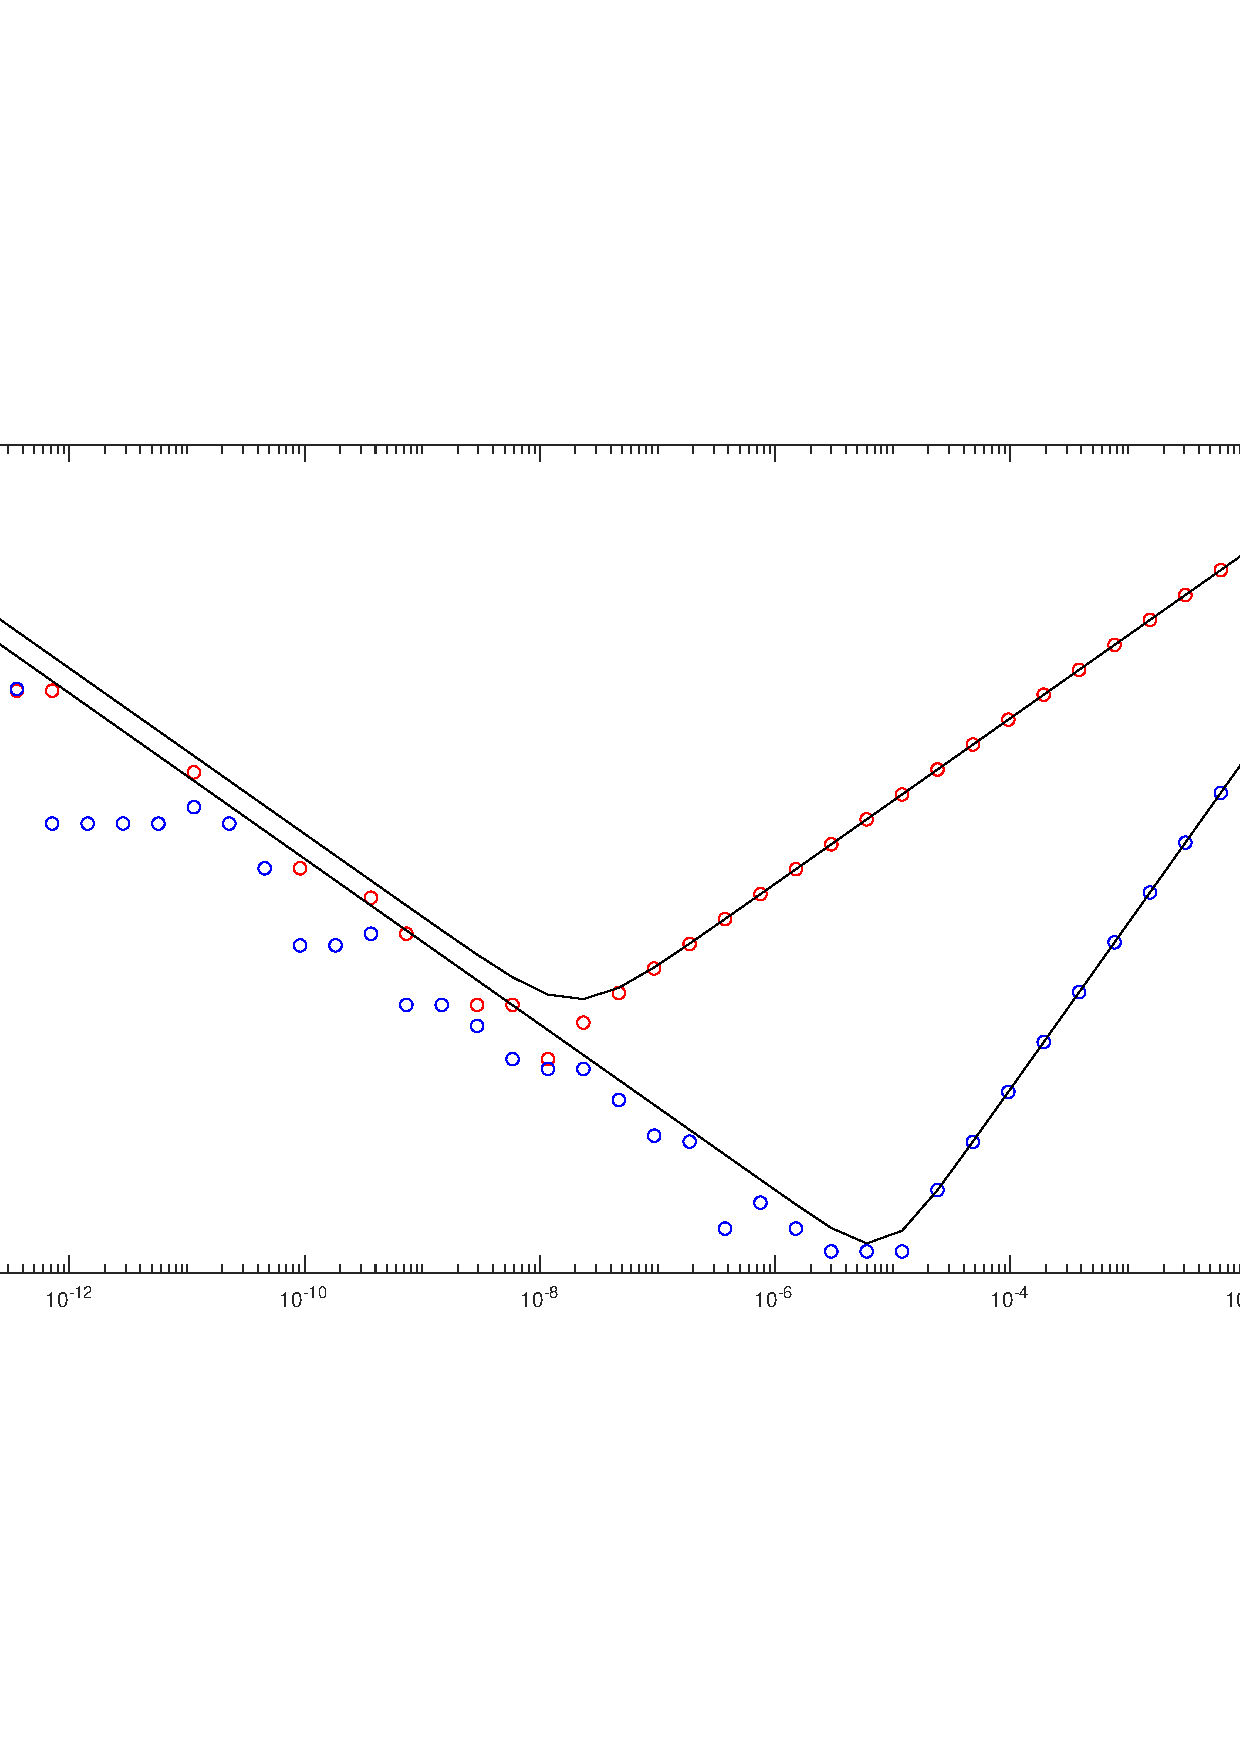
\includegraphics[width = 0.55\textwidth]{Sem_2_fig_1}
			\caption{Визуализация погрешностей вычисления на компьютере}
			\label{fig:fig_1}
		\end{figure}
	
	\section{Основы линейной алгебры}
	
		Вспомним основные понятия:
		
		\subsection{Норма}
		
			\begin{enumerate}
				\item $\parallel x\parallel \geq 0, \parallel x \parallel = 0 \Leftrightarrow x = 0$
				\item $\parallel \alpha x \parallel = \left|\alpha\right| \parallel x\parallel$
				\item $\parallel x + z \parallel \leq \parallel x+ y \parallel + \parallel y + z\parallel$
			\end{enumerate}
			
			\begin{equation}
				l_{p} = \sqrt[p]{\sum\limits_{i} x_{i}^{p}}
			\end{equation}
			
			Матричная норма:
			
			\begin{enumerate}
				\item $\parallel A\parallel \geq 0, \parallel A \parallel = 0 \Leftrightarrow A = 0$
				\item $\parallel \alpha A \parallel = \left|\alpha\right| \parallel A\parallel$
				\item $\parallel A + B \parallel \leq \parallel A + C \parallel + \parallel C + B\parallel$
				\item $\parallel AB\parallel \leq \parallel A\parallel \parallel B\parallel$
			\end{enumerate}
			
			Матричная норма Фробениуса:
			
			\begin{equation}
				\parallel A\parallel_{F} = \sqrt{\sum a_{ij}^{2}}
			\end{equation}
			
			Понятие подчиненной нормы:
			
			\begin{equation}
				\parallel A\parallel = \sup\limits_{x \neq 0} \frac{\parallel A x\parallel}{\parallel x\parallel}	= \max\limits_{\parallel y\parallel = 1} \parallel A y\parallel
			\end{equation}
			
			Рассмотрим некоторые виды норм:
			
			\begin{enumerate}
				\item $\parallel A\parallel_{1} = \max\limits_{j}\sum\limits_{i}\left|a_{ij}\right|$
				\item $\parallel A\parallel_{2} = \sqrt{\max\limits_{i}\lambda_{i}A^{T}A}$
				\item $\parallel A\parallel_{\infty} = \max\limits_{i}\sum\limits_{j}\left|a_{ij}\right|$
			\end{enumerate}						 
\end{document}